\documentclass[letterpaper, 10pt]{article}
\usepackage[utf8]{inputenc}
\usepackage{amsmath}
\usepackage{amsfonts}
\usepackage{amssymb}
\usepackage[letterpaper, margin=1in]{geometry}

\usepackage{pgfplots}
\usepackage{xcolor}
\usepackage{listings}
\usepackage{layouts}
\usepackage[section]{placeins}
\lstset{ 
	% language=Python,                	% choose the language of the code
	basicstyle=\ttfamily\footnotesize, 	% the size of the fonts that are used for the code
	numbers=left,                   	% where to put the line-numbers
	numberstyle=\ttfamily\footnotesize, % the size of the fonts that are used for the line-numbers
	stepnumber=1,                   	% the step between two line-numbers. If it is 1 each line will be numbered
	numbersep=5pt,                  	% how far the line-numbers are from the code
	backgroundcolor=\color{white}, 		% choose the background color. You must add \usepackage{color}
	showspaces=false,               	% show spaces adding particular underscores
	showstringspaces=false,         	% underline spaces within strings
	showtabs=false,                 	% show tabs within strings adding particular underscores
	frame=single,           			% adds a frame around the code
	tabsize=4,          				% sets default tabsize to 4 spaces
	captionpos=t,           			% sets the caption-position to bottom
	breaklines=true,        			% sets automatic line breaking
	breakatwhitespace=false,    		% sets if automatic breaks should only happen at whitespace
	escapeinside={\%*}{*)}          	% if you want to add a comment within your code
	% prebreak=\raisebox{0ex}[0ex][0ex]{\ensuremath{\hookleftarrow}})
}

% \pagenumbering{gobble}

\begin{document}
\section{Question 1}
\begin{figure}[h]
\centering
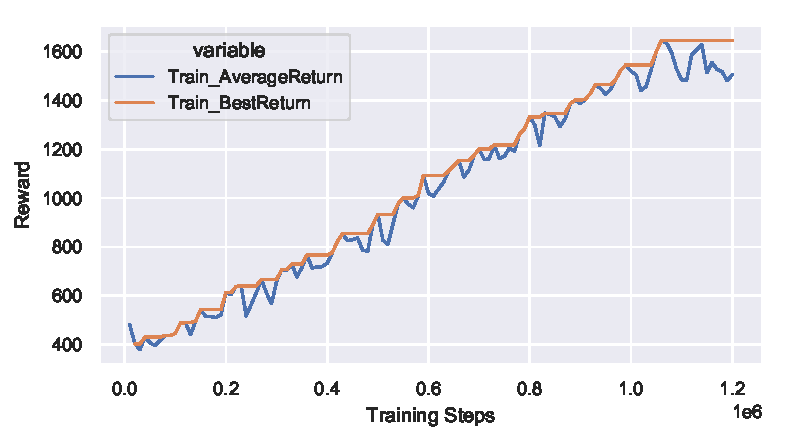
\includegraphics{figures/q1.pdf}
\caption{basic Q-learning performance}
\end{figure}

\begin{lstlisting}[caption=Exact command line configurations]
python cs285/scripts/run_hw3_dqn.py --env_name MsPacman-v0 --exp_name q1
\end{lstlisting}

\newpage

\section{Question 2}
\begin{figure}[h]
\centering
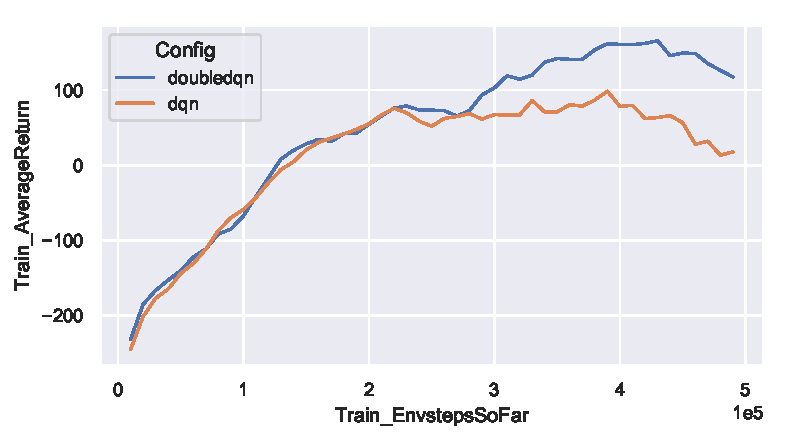
\includegraphics{figures/q2.pdf}
\caption{double Q-learning}
\end{figure}

\begin{lstlisting}[caption=Exact command line configurations]
python cs285/scripts/run_hw3_dqn.py --env_name LunarLander-v3 --exp_name q2_dqn_1 --seed 1
python cs285/scripts/run_hw3_dqn.py --env_name LunarLander-v3 --exp_name q2_dqn_2 --seed 2
python cs285/scripts/run_hw3_dqn.py --env_name LunarLander-v3 --exp_name q2_dqn_3 --seed 3

python cs285/scripts/run_hw3_dqn.py --env_name LunarLander-v3 --exp_name q2_doubledqn_1 --double_q --seed 1
python cs285/scripts/run_hw3_dqn.py --env_name LunarLander-v3 --exp_name q2_doubledqn_2 --double_q --seed 2
python cs285/scripts/run_hw3_dqn.py --env_name LunarLander-v3 --exp_name q2_doubledqn_3 --double_q --seed 3
\end{lstlisting}

As expected, double Q-learning does better than normal DQN. Note that the three runs for DQN and double DQN were averaged
together.

\newpage

\section{Question 3}
\begin{figure}[h]
\centering
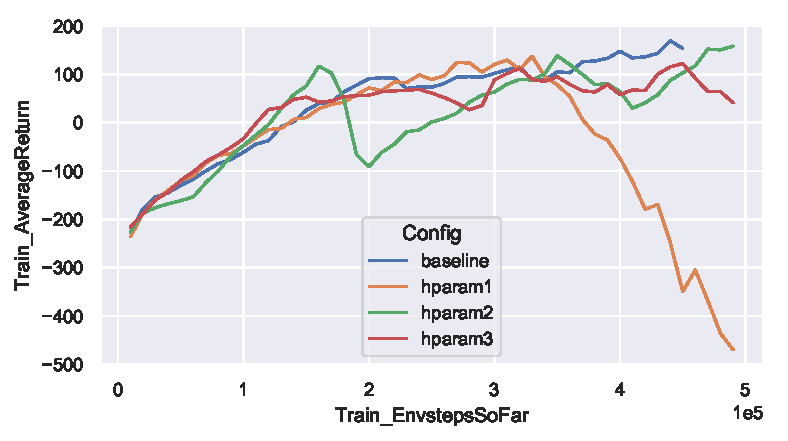
\includegraphics{figures/q3.pdf}
\caption{experimenting with hyperparameters }
\end{figure}
\begin{lstlisting}[caption=Exact command line configurations]
python cs285/scripts/run_hw3_dqn.py --env_name LunarLander-v3 --exp_name q3_hparam1
python cs285/scripts/run_hw3_dqn.py --env_name LunarLander-v3 --exp_name q3_hparam2
python cs285/scripts/run_hw3_dqn.py --env_name LunarLander-v3 --exp_name q3_hparam3
\end{lstlisting}

For this question, I experimented with the neural network architecture. The baseline is the default network architecture:
2 hidden layers, each of size 64. For \texttt{hparam1}, I increased the network size to 3 hidden layers, each with 64 units.
For \texttt{hparam2}, the network had 2 hidden layers, each of size 128. For \texttt{hparam3}, the network had 3 hidden layers,
each with 128 units. Most of these experiments performed similarly, except for \texttt{hparam1}, which looks to have diverged
and achieved a very negative reward!

\newpage

\section{Question 4}
\begin{figure}[h]
\centering
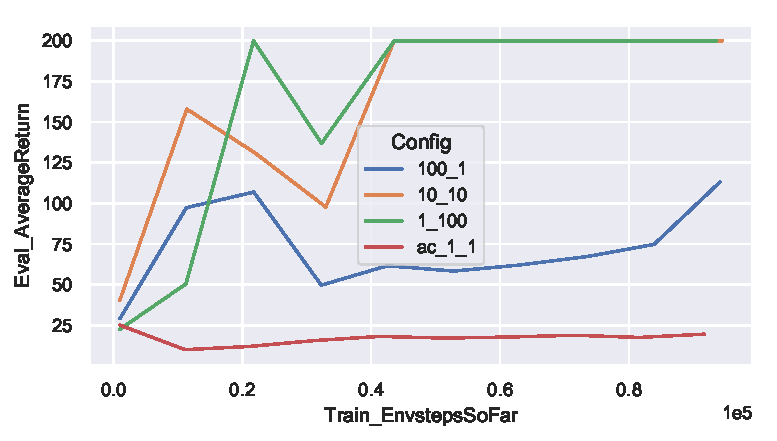
\includegraphics{figures/q4.pdf}
\caption{Sanity check with Cartpole}
\end{figure}

\begin{lstlisting}[caption=Exact command line configurations]
python run_hw3_actor_critic.py --env_name CartPole-v0 -n 100 -b 1000 --exp_name q4_ac_1_1 -ntu 1 -ngsptu 1
python run_hw3_actor_critic.py --env_name CartPole-v0 -n 100 -b 1000 --exp_name q4_100_1 -ntu 100 -ngsptu 1
python run_hw3_actor_critic.py --env_name CartPole-v0 -n 100 -b 1000 --exp_name q4_1_100 -ntu 1 -ngsptu 100
python run_hw3_actor_critic.py --env_name CartPole-v0 -n 100 -b 1000 --exp_name q4_10_10 -ntu 10 -ngsptu 10
\end{lstlisting}

From the graph, 10 target updates, each every 10 gradient steps and 1 target update, each every 100 gradient steps appear to
perform the best, although the single target update looks to converge faster, so I used those settings (\texttt{-ntu 1 -ngsptu 100})
to test on the harder tasks.

\newpage

\section{Question 5}
\begin{figure}[h]
\centering
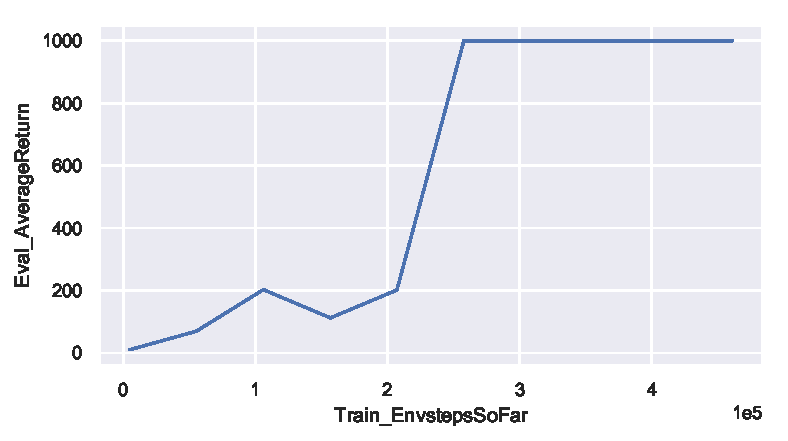
\includegraphics{figures/q5_inverted_pendulum.pdf}
\caption{Run actor-critic with more dicult tasks: \texttt{InvertedPendulum-v2}}
\end{figure}

\begin{lstlisting}[caption=Exact command line configurations]
python cs285/scripts/run_hw3_actor_critic.py --env_name InvertedPendulum-v2 --ep_len 1000 --discount 0.95 -n 100 -l 2 -s 64 -b 5000 -lr 0.01 --exp_name q5_1_100 -ntu 1 -ngsptu 100
\end{lstlisting}

\begin{figure}[h]
\centering
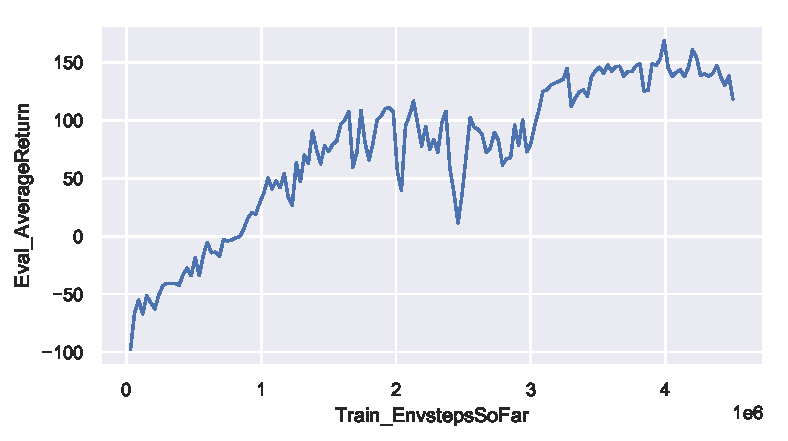
\includegraphics{figures/q5_half_cheetah.pdf}
\caption{Run actor-critic with more dicult tasks: \texttt{HalfCheetah-v2}}
\end{figure}

\begin{lstlisting}[caption=Exact command line configurations]
python cs285/scripts/run_hw3_actor_critic.py --env_name HalfCheetah-v2 --ep_len 150 --discount 0.90 --scalar_log_freq 1 -n 150 -l 2 -s 32 -b 30000 -eb 1500 -lr 0.02 --exp_name q5_1_100 -ntu 1 -ngsptu 100
\end{lstlisting}

\end{document}